\documentclass{beamer}
\usepackage{amsmath}
\usepackage[english]{babel} %set language; note: after changing this, you need to delete all auxiliary files to recompile
\usepackage[utf8]{inputenc} %define file encoding; latin1 is the other often used option
\usepackage{csquotes} % provides context sensitive quotation facilities
\usepackage{graphicx} %allows for inserting figures
\usepackage{booktabs} % for table formatting without vertical lines
\usepackage{textcomp} % allow for example using the Euro sign with \texteuro
\usepackage{stackengine}
\usepackage{wasysym}
\usepackage{tikzsymbols}
\usepackage{textcomp}
\usetikzlibrary{patterns} 
\usepackage{xcolor}
\usepackage[dvipsnames]{xcolor}
\usepackage{colortbl}
\usepackage{adjustbox}
\usetikzlibrary{shapes, arrows.meta, positioning}
% ELIMINAR COMANDOS DE NAVEGACION%%%%%%%%%%%
\setbeamertemplate{navigation symbols}

%\newcommand{\bubblethis}[2]{
 %       \tikz[remember picture,baseline]{\node[anchor=base,inner sep=0,outer sep=0]%
 %       (#1) {\underline{#1}};\node[overlay,cloud callout,callout relative pointer={(0.2cm,-0.7cm)},%
 %       aspect=2.5,fill=yellow!90] at ($(#1.north)+(-0.5cm,1.6cm)$) {#2};}%
 %   }%
%\tikzset{face/.style={shape=circle,minimum size=4ex,shading=radial,outer sep=0pt,
 %       inner color=white!50!yellow,outer color= yellow!70!orange}}

%% Some commands to make the code easier
\newcommand{\emoticon}[1][]{%
  \node[face,#1] (emoticon) {};
  %% The eyes are fixed.
  \draw[fill=white] (-1ex,0ex) ..controls (-0.5ex,0.2ex)and(0.5ex,0.2ex)..
        (1ex,0.0ex) ..controls ( 1.5ex,1.5ex)and( 0.2ex,1.7ex)..
        (0ex,0.4ex) ..controls (-0.2ex,1.7ex)and(-1.5ex,1.5ex)..
        (-1ex,0ex)--cycle;}
\newcommand{\pupils}{
  %% standard pupils
  \fill[shift={(0.5ex,0.5ex)},rotate=80] 
       (0,0) ellipse (0.3ex and 0.15ex);
  \fill[shift={(-0.5ex,0.5ex)},rotate=100] 
       (0,0) ellipse (0.3ex and 0.15ex);}

\newcommand{\emoticonname}[1]{
  \node[below=1ex of emoticon,font=\footnotesize,
        minimum width=4cm]{#1};}
\usepackage{scalerel}
\usetikzlibrary{positioning}
\usepackage{xcolor,amssymb}
\newcommand\dangersignb[1][2ex]{%
  \scaleto{\stackengine{0.3pt}{\scalebox{1.1}[.9]{%
  \color{red}$\blacktriangle$}}{\tiny\bfseries !}{O}{c}{F}{F}{L}}{#1}%
}
\newcommand\dangersignw[1][2ex]{%
  \scaleto{\stackengine{0.3pt}{\scalebox{1.1}[.9]{%
  \color{red}$\blacktriangle$}}{\color{white}\tiny\bfseries !}{O}{c}{F}{F}{L}}{#1}%
}
\usepackage{fontawesome} % Social Icons
\usepackage{epstopdf} % allow embedding eps-figures
\usepackage{tikz} % allows drawing figures
\usepackage{amsmath,amssymb,amsthm} %advanced math facilities
\usepackage{lmodern} %uses font that support italic and bold at the same time
\usepackage{hyperref}
\usepackage{tikz}
\hypersetup{
    colorlinks=true,
    linkcolor=blue,
    filecolor=magenta,      
    urlcolor=blue,
}
\usepackage{tcolorbox}
%add citation management using BibLaTeX
\usepackage[citestyle=authoryear-comp, %define style for citations
    bibstyle=authoryear-comp, %define style for bibliography
    maxbibnames=10, %maximum number of authors displayed in bibliography
    minbibnames=1, %minimum number of authors displayed in bibliography
    maxcitenames=3, %maximum number of authors displayed in citations before using et al.
    minnames=1, %maximum number of authors displayed in citations before using et al.
    datezeros=false, % do not print dates with leading zeros
    date=long, %use long formats for dates
    isbn=false,% show no ISBNs in bibliography (applies only if not a mandatory field)
    url=false,% show no urls in bibliography (applies only if not a mandatory field)
    doi=false, % show no dois in bibliography (applies only if not a mandatory field)
    eprint=false, %show no eprint-field in bibliography (applies only if not a mandatory field)
    backend=biber %use biber as the backend; backend=bibtex is less powerful, but easier to install
    ]{biblatex}
\addbibresource{../mybibfile.bib} %define bib-file located one folder higher


\usefonttheme[onlymath]{serif} %set math font to serif ones

\definecolor{beamerblue}{rgb}{0.2,0.2,0.7} %define beamerblue color for later use

%%% defines highlight command to set text blue
\newcommand{\highlight}[1]{{\color{blue}{#1}}}


%%%%%%% commands defining backup slides so that frame numbering is correct

\newcommand{\backupbegin}{
   \newcounter{framenumberappendix}
   \setcounter{framenumberappendix}{\value{framenumber}}
}
\newcommand{\backupend}{
   \addtocounter{framenumberappendix}{-\value{framenumber}}
   \addtocounter{framenumber}{\value{framenumberappendix}}
}

%%%% end of defining backup slides

%Specify figure caption, see also http://tex.stackexchange.com/questions/155738/caption-package-not-working-with-beamer
\setbeamertemplate{caption}{\insertcaption} %redefines caption to remove label "Figure".
%\setbeamerfont{caption}{size=\scriptsize,shape=\itshape,series=\bfseries} %sets figure  caption bold and italic and makes it smaller


\usetheme{Boadilla}

%set options of hyperref package
\hypersetup{
    bookmarksnumbered=true, %put section numbers in bookmarks
    naturalnames=true, %use LATEX-computed names for links
    citebordercolor={1 1 1}, %color of border around cites, here: white, i.e. invisible
    linkbordercolor={1 1 1}, %color of border around links, here: white, i.e. invisible
    colorlinks=true, %color links
    anchorcolor=black, %set color of anchors
    linkcolor=beamerblue, %set link color to beamer blue
    citecolor=blue, %set cite color to beamer blue
    pdfpagemode=UseThumbs, %set default mode of PDF display
    breaklinks=true, %break long links
    pdfstartpage=1 %start at first page
    }

\newtcolorbox{boxA}{
    fontupper = \bf,
    boxrule = 1.5pt,
    colframe = black % frame color
}
\newtcolorbox{boxB}{
    boxrule = 1.5pt,
    colframe = blue!70!black,, % frame color
    colback = blue!7!white,
}

% --------------------
% Overall information
% --------------------
\title[Economía I]{Economía I \vspace{3mm}
\\ Magistral 15 \vspace{3mm} \\ Competencia imperfecta}
\date{}
\author[Victoria Rosino]{Victoria Rosino}
\vspace{0.3cm}
\institute[]{Universidad de San Andrés} 

\begin{document}

\begin{frame}
\vspace{0.3cm}
\titlepage
\centering
\vspace{-0.9cm}

\includegraphics[scale=0.3]{Slides Principios de Economia/Figures/udesa_logo.jpg} 
\end{frame}

\begin{frame}
\frametitle{El problema de la firma}
\begin{itemize}
    \item Una vez que conocemos la demanda... ¿cómo se elige cuánto producir y qué precio cobrar?
    \vspace{1mm}
    \item El problema principal de \textbf{toda} empresa es el de la maximización del beneficio
    \vspace{1mm}     
    \begin{itemize}
        \item ¿Qué es el beneficio? \vspace{1mm} \\ 
        Beneficio = Ingresos totales – Costos totales
        \vspace{1mm}
        \item ¿Qué es el ingreso total? 
        \vspace{1mm} \\ 
        El valor de la producción al precio ofrecido ($p\cdot q$)
        \vspace{1mm}
        \item ¿Qué es el costo total?
        \vspace{1mm} \\ 
        Los costos por unidad, por la cantidad de unidades producidas ($c\cdot q$)
    \end{itemize} 
\end{itemize} 
\end{frame}

\begin{frame}
\frametitle{Estructuras de mercado}
  \begin{itemize} 
    \item En \textbf{competencia perfecta}, las empresas eran tomadoras de precios y \textbf{solo eligen la cantidad} que producen maximizando sus beneficios ($P=CMg$). \vspace{1mm}
     \item  La \textbf{competencia imperfecta} se hace presente cuando existe una o varias empresas que tienen la habilidad de \textbf{controlar}, en alguna medida, el \textbf{precio} de su producto. \vspace{1mm}
     \item El monopolio no solo es el caso opuesto a la competencia perfecta, también es el caso extremo de las estructuras de mercado de competencia imperfecta. \vspace{1mm}
  \end{itemize} 
\end{frame}
\begin{frame}
\frametitle{Monopolio}
\begin{itemize}
    \item Hay una única empresa que vende productos especializados y tiene un alto poder de mercado. \vspace{1mm}
    \begin{itemize}
        \item Enfrenta poca (o nula) competencia, por lo que se enfrenta  a toda la curva de demanda del mercado.
       \item Enfrenta una demanda inelástica (no hay sustitutos cercanos) y puede fijar precio superior al costo marginal sin perder todos sus clientes. \vspace{1mm}
        \item Las barreras de entrada ayudan a generar rentas: 
            \begin{itemize}
               \item Beneficios económicos por encima de los costos de producción.
                \item Por eso las barreras a la entrada ¡son el peor enemigo de los economistas! (y de la sociedad)
            \end{itemize}
    \end{itemize}
    \vspace{1.5mm}
    \item En estos casos, en equilibrio encontramos una pérdida de peso muerto 
    \vspace{-4mm}
    \begin{itemize}
        \item Tenemos entonces una falla de mercado.
        \item Es decir, los mercados asignan recursos, sin competencia, en una forma no óptima. 
    \end{itemize}
    \end{itemize}
\end{frame}


\begin{frame}
\frametitle{Mirando el ingreso total}
\begin{itemize}
    \item Como el monopolista se enfrenta a toda la demanda, su pendiente negativa anticipa que el ingreso total irá variando a medida que varíen los precios, y por ende, las cantidades. \vspace{1mm}
    \item El concepto clave para la decisión del monopolista es el de ingreso marginal: \vspace{1mm}
    \begin{itemize}
        \item Es decir, la variación en los ingresos totales al vender una unidad adicional.
        \item Es el efecto neto de la disminución de los precios y el aumento de la cantidad vendida.\vspace{1mm}
    \end{itemize}
    \item La curva de demanda, veremos, nos determina ingresos marginales decrecientes. \vspace{1mm}
     \item ¿Cómo cambia el ingreso al aumentar la producción?
    \begin{itemize}
        \item Ahora se vende una unidad más... \\
        \item ...¡pero todas las vendo a un precio menor!
    \end{itemize}
\end{itemize}
\end{frame}

\begin{frame}
\frametitle{¿Cómo cambia el ingreso total?}

\begin{minipage}{0.45\textwidth}
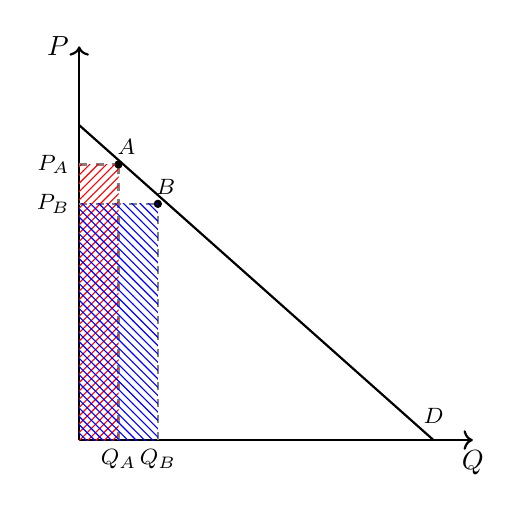
\begin{tikzpicture}[scale=1]
    \draw[thick,->] (0,0) -- (5,0) node[below] {$Q$};
    \draw[thick,->] (0,0) -- (0,5) node[left] {$P$};
    \draw[thick] (0,4) -- (4.5,0); 
    \node at (4.5,0.3) {\footnotesize $D$};

    \draw[thick, dashed, gray] (0,3.5) -- (0.5,3.5);
    \draw[thick, dashed, gray] (0.5,0) -- (0.5,3.5);
    \node[left] at (0,3.5) {\footnotesize $P_A$};
    \node[below] at (0.5,0) {\footnotesize $Q_A$};
    \fill (0.5,3.5) circle (1.5pt);
    \node [above] at (0.6,3.5) {\footnotesize $A$};

    \draw[thick, dashed, gray] (0,3) -- (1,3);
    \draw[thick, dashed, gray] (1,0) -- (1,3);
    \node[left] at (0,3) {\footnotesize $P_B$};
    \node[below] at (1,0) {\footnotesize $Q_B$};
    \fill (1,3) circle (1.5pt);
    \node [above] at (1.1,3) {\footnotesize $B$};

    \fill[pattern=north east lines,  pattern color=red] (0,0) rectangle (0.5,3.5);

    \fill[pattern=north west lines,  pattern color=blue] (0,0) rectangle (1,3);

\end{tikzpicture}
\end{minipage}
\hfill
\begin{minipage}{0.53\textwidth}
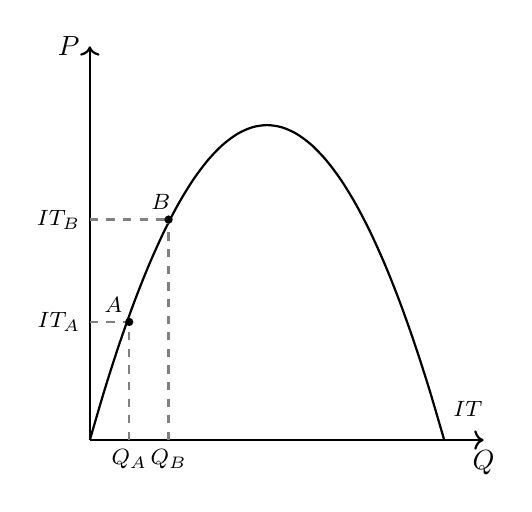
\begin{tikzpicture}[scale=1]
    \draw[thick,->] (0,0) -- (5,0) node[below] {$Q$};
    \draw[thick,->] (0,0) -- (0,5) node[left] {$P$};

%Parabola 
\draw[thick, domain=0:4.5, smooth, variable=\x] plot ({\x},{-0.79*(\x-2.25)^2+4});
\node at (4.8,0.4) {\footnotesize $IT$};


\draw[thick, dashed, gray] (0,1.5) -- (0.5,1.5);
\draw[thick, dashed, gray] (0.5,0) -- (0.5,1.5);
\fill (0.5,1.5) circle (1.5pt);
\node [above] at (0.3,1.5) {\footnotesize $A$};
\node[left] at (0,1.5) {\footnotesize $IT_A$};
\node[below] at (0.5,0) {\footnotesize $Q_A$};


\draw[thick, dashed, gray] (0,2.8) -- (1,2.8);
\draw[thick, dashed, gray] (1,0) -- (1,2.8);
\fill (1,2.8) circle (1.5pt);
\node [above] at (0.9,2.8) {\footnotesize $B$};
\node[left] at (0,2.8) {\footnotesize $IT_B$};
\node[below] at (1,0) {\footnotesize $Q_B$};


\end{tikzpicture}
\end{minipage}

\end{frame}

\begin{frame}
\frametitle{¿Cómo cambia el ingreso total?}

\begin{minipage}{0.45\textwidth}
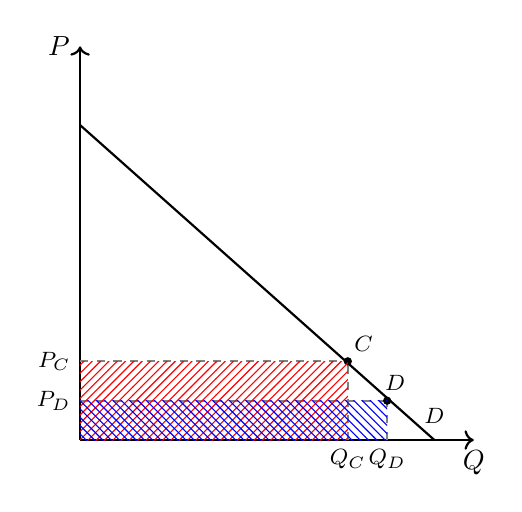
\begin{tikzpicture}[scale=1]
    \draw[thick,->] (0,0) -- (5,0) node[below] {$Q$};
    \draw[thick,->] (0,0) -- (0,5) node[left] {$P$};
    \draw[thick] (0,4) -- (4.5,0); 
    \node at (4.5,0.3) {\footnotesize $D$};

    \draw[thick, dashed, gray] (0,1) -- (3.4,1);
    \draw[thick, dashed, gray] (3.4,0) -- (3.4,1);
    \node[left] at (0,1) {\footnotesize $P_C$};
    \node[below] at (3.4,0) {\footnotesize $Q_C$};
    \fill (3.4,1) circle (1.5pt);
    \node [above] at (3.6,1) {\footnotesize $C$};

    \draw[thick, dashed, gray] (0,0.5) -- (3.9,0.5);
    \draw[thick, dashed, gray] (3.9,0) -- (3.9,0.5);
    \node[left] at (0,0.5) {\footnotesize $P_D$};
    \node[below] at (3.9,0) {\footnotesize $Q_D$};
    \fill (3.9,0.5) circle (1.5pt);
    \node [above] at (4,0.5) {\footnotesize $D$};

    \fill[pattern=north east lines,  pattern color=red] (0,0) rectangle (3.4,1);

    \fill[pattern=north west lines,  pattern color=blue] (0,0) rectangle (3.9,0.5);

\end{tikzpicture}
\end{minipage}
\hfill
\begin{minipage}{0.53\textwidth}
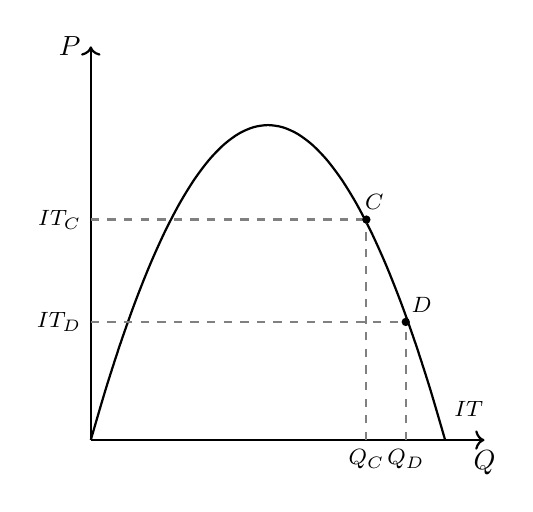
\begin{tikzpicture}[scale=1]
    \draw[thick,->] (0,0) -- (5,0) node[below] {$Q$};
    \draw[thick,->] (0,0) -- (0,5) node[left] {$P$};

%Parabola 
\draw[thick, domain=0:4.5, smooth, variable=\x] plot ({\x},{-0.79*(\x-2.25)^2+4});
\node at (4.8,0.4) {\footnotesize $IT$};


\draw[thick, dashed, gray] (0,1.5) -- (4,1.5);
\draw[thick, dashed, gray] (4,0) -- (4,1.5);
\fill (4,1.5) circle (1.5pt);
\node [above] at (4.2,1.5) {\footnotesize $D$};
\node[left] at (0,1.5) {\footnotesize $IT_D$};
\node[below] at (4,0) {\footnotesize $Q_D$};


\draw[thick, dashed, gray] (0,2.8) -- (3.5,2.8);
\draw[thick, dashed, gray] (3.5,0) -- (3.5,2.8);
\fill (3.5,2.8) circle (1.5pt);
\node [above] at (3.6,2.8) {\footnotesize $C$};
\node[left] at (0,2.8) {\footnotesize $IT_C$};
\node[below] at (3.5,0) {\footnotesize $Q_C$};

\end{tikzpicture}
\end{minipage}
\end{frame}


\begin{frame}
\frametitle{El ingreso marginal}
\begin{figure}[h!]
\centering
\scalebox{0.5}{
\tikzset{every picture/.style={line width=0.75pt}} %set default line width to 0.75pt        

\begin{tikzpicture}[x=0.75pt,y=0.75pt,yscale=-1,xscale=1]
%uncomment if require: \path (0,1344); %set diagram left start at 0, and has height of 1344

%Straight Lines [id:da18243805432710514] 
\draw    (202,871.69) -- (406,1108.5) ;
%Shape: Parabola [id:dp7498100266891665] 
\draw  [color={rgb, 255:red, 0; green, 0; blue, 0 }  ,draw opacity=1 ][line width=0.75]  (201,819.5) .. controls (269.33,562.42) and (337.67,562.42) .. (406,819.5) ;
%Straight Lines [id:da26559851992662464] 
\draw[->]    (201,821.69) -- (472,821.69) ;

%Straight Lines [id:da5363525623734258] 
\draw[->]    (201,1107.69) -- (472,1107.69) ;

%Straight Lines [id:da3817553551786188] 
\draw[->]    (201,821.69) -- (201,591.69) ;

%Straight Lines [id:da7748677219246147] 
\draw[->]    (201,1107.69) -- (200.01,854.69) ;


%Straight Lines [id:da4368467901848765] 
\draw    (202,871.69) -- (362,1231.69) ;
%Straight Lines [id:da5238163933422064] 
\draw    (303.5,626.69) -- (305,1107.69) ;

\fill (304,990.09) circle (3pt);
\fill (303.5,626.69) circle (3pt);
%Straight Lines [id:da3583437704153747] 
\draw[dashed]    (201,989.69) -- (304,990.09) ;
%Straight Lines [id:da11618331349069289] 
\draw[dashed]    (202,626.69) -- (303.5,626.69) ;

% Text Node
\draw (474,1110.69) node [anchor=north west][inner sep=0.75pt]   [align=left] {$Q$};
% Text Node
\draw (474,821.69) node [anchor=north west][inner sep=0.75pt]   [align=left] {$Q$};
% Text Node
\draw (118,576.69) node [anchor=north west][inner sep=0.75pt]   [align=left] {Ingreso total};
% Text Node
\draw (150,832.69) node [anchor=north west][inner sep=0.75pt]   [align=left] {Precio};
% Text Node
\draw (177,978.69) node [anchor=north west][inner sep=0.75pt]   [align=left] {$P_E$};
% Text Node
\draw (294,825.69) node [anchor=north west][inner sep=0.75pt]   [align=left] {$Q_E$};
% Text Node
\draw (407,1083.69) node [anchor=north west][inner sep=0.75pt]   [align=left] {$D$};
% Text Node
\draw (409,785.69) node [anchor=north west][inner sep=0.75pt]   [align=left] {$IT$};
% Text Node
\draw (343,1160.69) node [anchor=north west][inner sep=0.75pt]   [align=left] {$IMg$};
% Text Node
\draw (298,602) node [anchor=north west][inner sep=0.75pt]   [align=left] {{ $E$}};
% Text Node
\draw (291,1110.69) node [anchor=north west][inner sep=0.75pt]   [align=left] {$Q_E$};
% Text Node
\draw (306,967) node [anchor=north west][inner sep=0.75pt]   [align=left] {{$E$}};
% Text Node
\draw (137,620.69) node [anchor=north west][inner sep=0.75pt]   [align=left] {Ingreso \ \\máximo};

\end{tikzpicture}
}
\end{figure}
\end{frame}

\begin{frame}
\frametitle{El ingreso marginal}
\centering
\begin{tikzpicture}[scale=1.3]
    \draw[thick,->] (0,0) -- (5,0) node[below] {$Q$};
    \draw[thick,->] (0,0) -- (0,5) node[left] {$P$};
    \draw[thick] (0,4) -- (4.5,0); 
    \node at (4.5,0.3) {\footnotesize $D$};
    %IMg
    \draw[thick, blue] (0,4) -- (2.7,-0.7); 
    \node[blue] at (2.9,-0.5) {\footnotesize $IMg$};
    \end{tikzpicture}
\end{frame}

%\begin{frame}
%\frametitle{Costo e ingreso marginal}
%\centering
%\begin{tikzpicture}[scale=1.3]
%    \draw[thick,->] (0,0) -- (5,0) node[below] {$Q$};
%    \draw[thick,->] (0,0) -- (0,5) node[left] {$P$};
%    \draw[thick] (0,4) -- (4.5,0); 
%    \node at (4.5,0.3) {\footnotesize $D$};
    
%IMg
%\draw[thick, blue] (0,4) -- (2.25,0); 
%\node[blue] at (2.5,0.3) {\footnotesize $IMg$};

% Costo medio 
%\draw[thick] (0,3.2)..controls (2.2,1.5) and (3,1.5) .. (5.5,3.2)node[above right] {\footnotesize $CMe$};

% Costo marginal 
%\draw[thick,BlueGreen, domain=0.3:4, smooth, variable=\x] plot ({\x},{0.25*\x*\x}) node[above right, BlueGreen] {\footnotesize $CMg$};

%\end{tikzpicture}
%\end{frame}

\begin{frame}
\frametitle{Costo e ingreso marginal}
\centering
\tikzset{every picture/.style={line width=0.75pt}}   

\begin{tikzpicture}[x=0.75pt,y=0.75pt,yscale=-1,xscale=1]

%Straight Lines [id:da6898288131267385] 
\draw[->]    (94,318) -- (364,318) ;
%Straight Lines [id:da9536118190051617] (eje Y)
\draw[->]    (94,318) -- (94,68) ;
%Straight Lines [id:da07757000222951138] (demanda)
\draw    (95,91) -- (341,317) ;
%Curve Lines [id:da3185207500621865] 
\draw    (114,168) .. controls (147,254) and (275,246) .. (302,165) ;
%Straight Lines [id:da6853761324294885] (IMg)
\draw[blue]    (95,91) -- (230,350) ;
%Curve Lines [id:da24417480382196666] 
\draw[BlueGreen]    (116,316) .. controls (158,301) and (256,179) .. (281,133) ;

% Text Node
\draw (77,66) node [anchor=north west][inner sep=0.75pt]   [align=left] {\small $P$};
% Text Node
\draw (366,318) node [anchor=north west][inner sep=0.75pt]   [align=left] {\small $Q$};
% Text Node
\draw (302,155) node [anchor=north west][inner sep=0.75pt]   [align=left] {\footnotesize $CMeT$};
% Text Node
\draw[BlueGreen] (281,120) node [anchor=north west][inner sep=0.75pt]   [align=left] {\footnotesize $CMg$};
% Text Node
% Text Node
% Text Node
\draw[blue] (225,330) node [anchor=north west][inner sep=0.75pt]   [align=left] {\footnotesize $IMg$};
% Text Node
\draw (337,292) node [anchor=north west][inner sep=0.75pt]   [align=left] {\footnotesize $D$};

\end{tikzpicture}

\end{frame}


%\begin{frame}
%\frametitle{Maximización de beneficios}
%\centering
%\begin{tikzpicture}[scale=1.3]
 %   \draw[thick,->] (0,0) -- (5,0) node[below] {$Q$};
 %   \draw[thick,->] (0,0) -- (0,5) node[left] {$P$};
 %   \draw[thick] (0,4) -- (4.5,0); 
 %   \node at (4.5,0.3) {\footnotesize $D$};
    
%IMg
%\draw[thick, blue] (0,4) -- (2.25,0); 
%\node[blue] at (2.5,0.3) {\footnotesize $IMg$};
% Costo medio 
%\draw[thick] (0,2.7)..controls (2,1) and (3,1) .. (5.5,2.7)node[above right] {\footnotesize $CMe$};
% Costo marginal 
%\draw[thick, BlueGreen, domain=0.3:4, smooth, variable=\x] plot ({\x},{0.25*\x*\x}) node[above right] {\footnotesize $CMg$};

% Línea punteada desde punto de equilibrio
%\draw[dashed] (1.8,0) -- (1.8,2.4);
%\draw[dashed] (0,2.4) -- (1.8,2.4);
%\draw[dashed] (0,1.55) -- (1.8,1.55);

% Punto de intersección
%\filldraw (1.8,0.8) circle (1.5pt);

% Etiqueta de p*
%\node[left] at (0,2.4) {\footnotesize $P_M$};
%\node[left] at (0,1.55) {\footnotesize $CMeT$};

%\fill[green!70!black, opacity=0.3] (0,1.55) rectangle (1.8,2.4);

%\end{tikzpicture}
%\end{frame}

\begin{frame}
\frametitle{Maximización de beneficios}
\centering
\tikzset{every picture/.style={line width=0.75pt}}   

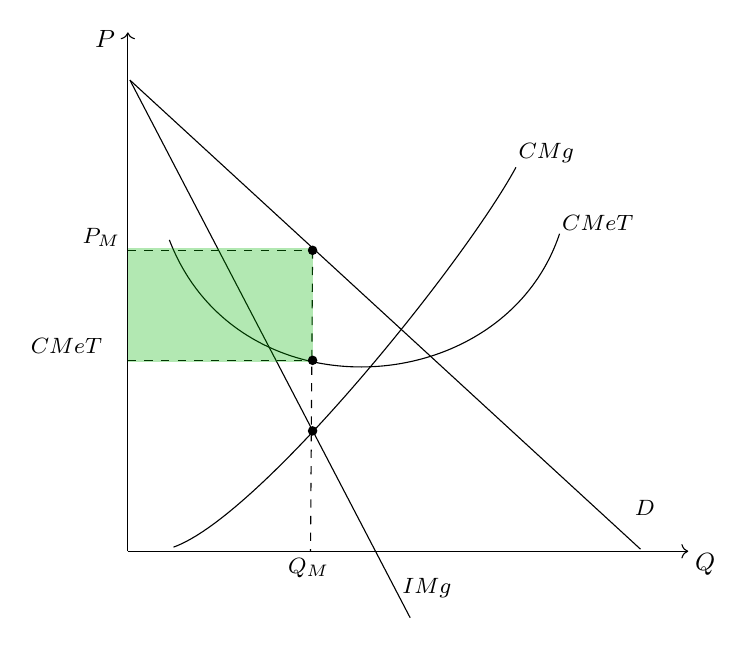
\begin{tikzpicture}[x=0.75pt,y=0.75pt,yscale=-1,xscale=1]

%Straight Lines [id:da6898288131267385] 
\draw[->]    (94,318) -- (364,318) ;
%Straight Lines [id:da9536118190051617] (eje Y)
\draw[->]    (94,318) -- (94,68) ;
%Straight Lines [id:da07757000222951138] (demanda)
\draw    (95,91) -- (341,317) ;
%Curve Lines [id:da3185207500621865] 
\draw    (114,168) .. controls (147,254) and (275,246) .. (302,165) ;
%Straight Lines [id:da9356870159511061] 
\draw[dashed]    (183,173) -- (182,318) ;
%Straight Lines [id:da6853761324294885] (IMg)
\draw    (95,91) -- (230,350) ;
%Straight Lines [id:da5731211677031389] 
\draw[dashed]    (94,173) -- (183,173) ;
%Straight Lines [id:da382163957096882] 
\draw[dashed]    (94,226) -- (183,226) ;
%Shape: Rectangle [id:dp41047149663713345] 
\fill[green!70!black, opacity=0.3] (94,172)  rectangle (183,227);

%Curve Lines [id:da24417480382196666] (CMg)
\draw    (116,316) .. controls (158,301) and (256,179) .. (281,133) ;

% Text Node
\draw (77,66) node [anchor=north west][inner sep=0.75pt]   [align=left] {\small $P$};
% Text Node
\draw (366,318) node [anchor=north west][inner sep=0.75pt]   [align=left] {\small $Q$};
% Text Node
\draw (302,155) node [anchor=north west][inner sep=0.75pt]   [align=left] {\footnotesize $CMeT$};
% Text Node
\draw (281,120) node [anchor=north west][inner sep=0.75pt]   [align=left] {\footnotesize $CMg$};
% Text Node
\draw (71,161) node [anchor=north west][inner sep=0.75pt]   [align=left] {\footnotesize $P_M$};
% Text Node
\draw (170,320) node [anchor=north west][inner sep=0.75pt]   [align=left] {\footnotesize $Q_M$};
% Text Node
\draw (46,214) node [anchor=north west][inner sep=0.75pt]   [align=left] {\footnotesize $CMeT$};
% Text Node
\draw (225,330) node [anchor=north west][inner sep=0.75pt]   [align=left] {\footnotesize $IMg$};
% Text Node
\draw (337,292) node [anchor=north west][inner sep=0.75pt]   [align=left] {\footnotesize $D$};

\filldraw (183,173) circle (1.5pt);
\filldraw (183,226) circle (1.5pt);
\filldraw (183,260) circle (1.5pt);

\end{tikzpicture}
\end{frame}


\begin{frame}
\frametitle{La lógica marginal}
\begin{itemize}
    \item El punto que maximiza el beneficio es donde la curva de IMg cruza la curva de CMg. \vspace{2mm}
    \item Recordemos que: 
     \[ B = p \cdot q \ – \ C(q) = IT(q) - C(q)\] \vspace{-4mm}
        \begin{itemize}
        \item Para cualquier valor de $q$, el cambio del beneficio si $q$ fuera aumentado en una unidad sería la diferencia entre el cambio en ingresos, y el cambio en costos: \vspace{2mm}  
        \begin{center} 
            Beneficio marginal = IMg - CMg 
            \end{center}
        \vspace{2mm}
        \item Entonces: 
         \begin{itemize}
            \item  Si $IMg > CMg$ aumentando $q$ se podrían incrementar los beneficios.
            \item  Si $IMg < CMg$ el beneficio marginal es negativo, con lo que sería mejor disminuir $q$ para aumentar los beneficios.
             \end{itemize}
    \end{itemize}
    \end{itemize}
\end{frame}


\begin{frame}
\frametitle{Mark-up}
\begin{itemize}
    \item La diferencia vertical entre el precio y el costo marginal ($P_M-CMg$) para $Q_M$ la llamamos \textbf{margen de beneficios}. \vspace{1mm}
    \item  Si expresamos esa diferencia como porcentaje del precio ($\frac{P-CMg}{P}$), entonces obtenemos el \textbf{mark-up}, es decir, el porcentaje de ganancia por arriba del costo marginal. \vspace{1mm}
    \item El mark-up es un \textbf{indicador del poder de mercado} de una empresa. 
    \begin{itemize}
        \item  Noten que en competencia perfecta, el equilibrio estaba cuando ($P=CMg$). Es decir, el mark-up es cero! Las empresas no tienen poder de mercado! \vspace{1mm}
    \end{itemize}
    \end{itemize}
\end{frame}

\begin{frame}
\frametitle{Excedentes y peso muerto}
\begin{itemize}
    \item Las ganancias totales del intercambio están determinadas por los excedentes de consumidores y productores.
    \begin{itemize}
        \item El excedente del consumidor: Diferencia entre disposición a pagar y precio de compra.  
        \item Excedente del productor: Diferencia entre precio y costo de una unidad adicional. \vspace{2mm}
    \end{itemize}
    \item Si no terminamos en una asignación Pareto eficiente tenemos una \textbf{pérdida de peso muerto}.
    \begin{itemize}
        \item Pérdida de excedente total con respecto a una asignación Pareto eficiente. Es decir, hay ganancias no explotadas del comercio.
    \end{itemize}
    \end{itemize}
\end{frame}

%\begin{frame}
%\frametitle{Precios y excedentes}
%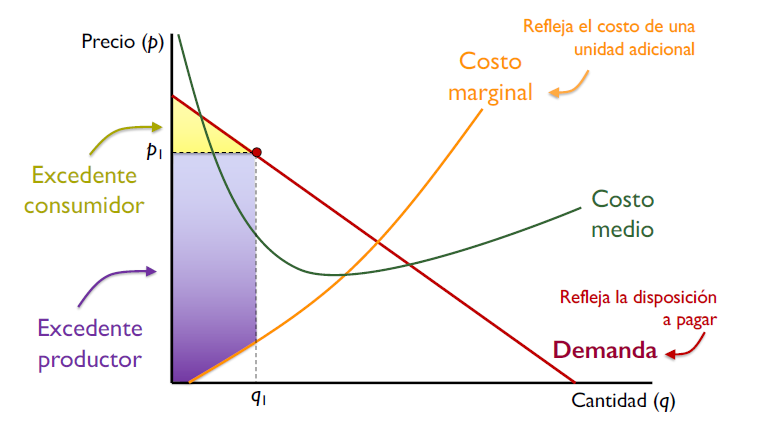
\includegraphics[scale=0.6]{Slides Principios de Economia/Figures/Tema_06.38_excedente1.png}
%\end{frame}

%\begin{frame}
%\frametitle{Mejora de Pareto}
%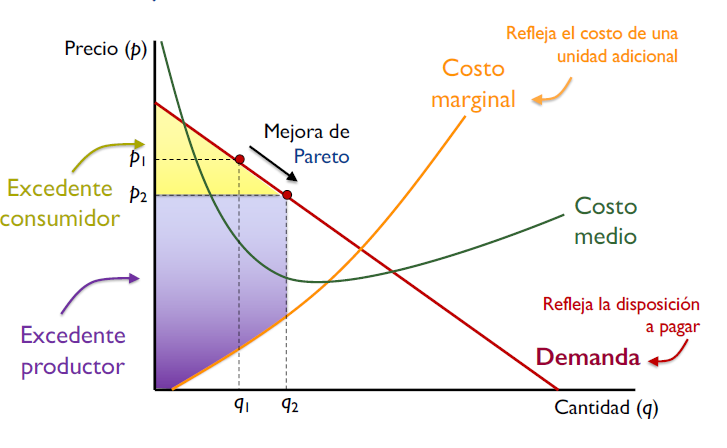
\includegraphics[scale=0.6]{Slides Principios de Economia/Figures/Tema_06.39_excedente2.png}
%\end{frame}

\begin{frame}
\frametitle{Excedentes en el caso monopolista}
\tikzset{every picture/.style={line width=0.75pt}}   
\centering
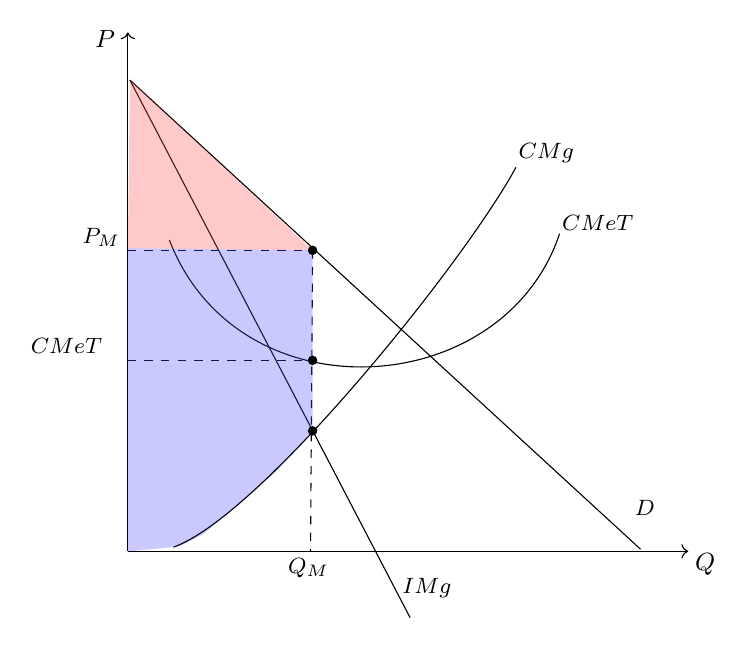
\begin{tikzpicture}[x=0.75pt,y=0.75pt,yscale=-1,xscale=1]

%Straight Lines [id:da6898288131267385] 
\draw[->]    (94,318) -- (364,318) ;
%Straight Lines [id:da9536118190051617] (eje Y)
\draw[->]    (94,318) -- (94,68) ;
%Straight Lines [id:da07757000222951138] (demanda)
\draw    (95,91) -- (341,317) ;
%Curve Lines [id:da3185207500621865] 
\draw    (114,168) .. controls (147,254) and (275,246) .. (302,165) ;
%Straight Lines [id:da9356870159511061] 
\draw[dashed]    (183,173) -- (182,318) ;
%Straight Lines [id:da6853761324294885] (IMg)
\draw    (95,91) -- (230,350) ;
%Straight Lines [id:da5731211677031389] 
\draw[dashed]    (94,173) -- (183,173) ;
%Straight Lines [id:da382163957096882] 
\draw[dashed]    (94,226) -- (183,226) ;

%EC
\fill[red!70, opacity=0.3] (94,172) --  (95,91) -- (183,173) -- cycle;

%EP
\fill[blue!70, opacity=0.3] (94,318) -- (94,172) -- (183,173) -- (183,260) -- (165,280) -- (130,310) -- (120,315) -- (116,316) -- cycle;

%Curve Lines [id:da24417480382196666] (CMg)
\draw    (116,316) .. controls (158,301) and (256,179) .. (281,133) ;

% Text Node
\draw (77,66) node [anchor=north west][inner sep=0.75pt]   [align=left] {\small $P$};
% Text Node
\draw (366,318) node [anchor=north west][inner sep=0.75pt]   [align=left] {\small $Q$};
% Text Node
\draw (302,155) node [anchor=north west][inner sep=0.75pt]   [align=left] {\footnotesize $CMeT$};
% Text Node
\draw (281,120) node [anchor=north west][inner sep=0.75pt]   [align=left] {\footnotesize $CMg$};
% Text Node
\draw (71,161) node [anchor=north west][inner sep=0.75pt]   [align=left] {\footnotesize $P_M$};
% Text Node
\draw (170,320) node [anchor=north west][inner sep=0.75pt]   [align=left] {\footnotesize $Q_M$};
% Text Node
\draw (46,214) node [anchor=north west][inner sep=0.75pt]   [align=left] {\footnotesize $CMeT$};
% Text Node
\draw (225,330) node [anchor=north west][inner sep=0.75pt]   [align=left] {\footnotesize $IMg$};
% Text Node
\draw (337,292) node [anchor=north west][inner sep=0.75pt]   [align=left] {\footnotesize $D$};

\filldraw (183,173) circle (1.5pt);
\filldraw (183,226) circle (1.5pt);
\filldraw (183,260) circle (1.5pt);

\end{tikzpicture}
\end{frame}

\begin{frame}
\frametitle{Eficiencia de Pareto}
\tikzset{every picture/.style={line width=0.75pt}}   
\centering
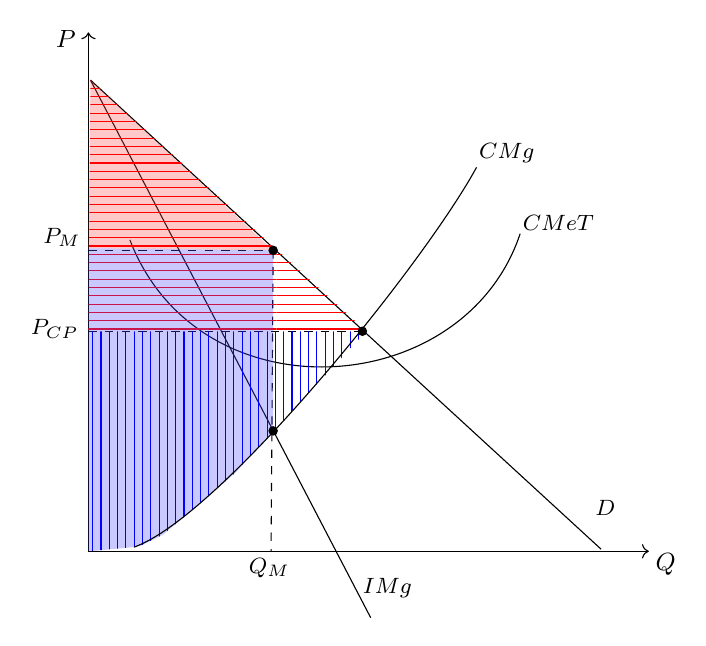
\begin{tikzpicture}[x=0.75pt,y=0.75pt,yscale=-1,xscale=1]

%Straight Lines [id:da6898288131267385] 
\draw[->]    (94,318) -- (364,318) ;
%Straight Lines [id:da9536118190051617] (eje Y)
\draw[->]    (94,318) -- (94,68) ;
%Straight Lines [id:da07757000222951138] (demanda)
\draw    (95,91) -- (341,317) ;
%Curve Lines [id:da3185207500621865] 
\draw    (114,168) .. controls (147,254) and (275,246) .. (302,165) ;
%Straight Lines [id:da9356870159511061] 
\draw[dashed]    (183,173) -- (182,318) ;
%Straight Lines [id:da6853761324294885] (IMg)
\draw    (95,91) -- (230,350) ;
%Straight Lines [id:da5731211677031389] 
\draw[dashed]    (94,173) -- (183,173) ;
%Straight Lines [id:da382163957096882] 
\draw[dashed]    (94,212) -- (226,212) ;


%EC
\fill[red!70, opacity=0.3] (94,172) --  (95,91) -- (183,173) -- cycle;
\fill[pattern=horizontal lines,  pattern color=red] (95,91) -- (228,212) -- (94,212) -- cycle;

%EP
\fill[blue!70, opacity=0.3] (94,318) -- (94,172) -- (183,173) -- (183,260) -- (165,280) -- (130,310) -- (120,315) -- (116,316) -- cycle;

\fill[pattern=vertical lines,  pattern color=blue]  (94,212) -- (228,212) -- (183,260) -- (165,280) -- (130,310) -- (120,315) -- (116,316) -- (94,318) -- cycle;

%Curve Lines [id:da24417480382196666] (CMg)
\draw    (116,316) .. controls (158,301) and (256,179) .. (281,133) ;

% Text Node
\draw (77,66) node [anchor=north west][inner sep=0.75pt]   [align=left] {\small $P$};
% Text Node
\draw (366,318) node [anchor=north west][inner sep=0.75pt]   [align=left] {\small $Q$};
% Text Node
\draw (302,155) node [anchor=north west][inner sep=0.75pt]   [align=left] {\footnotesize $CMeT$};
% Text Node
\draw (281,120) node [anchor=north west][inner sep=0.75pt]   [align=left] {\footnotesize $CMg$};
% Text Node
\draw (71,161) node [anchor=north west][inner sep=0.75pt]   [align=left] {\footnotesize $P_M$};
% Text Node
\draw (170,320) node [anchor=north west][inner sep=0.75pt]   [align=left] {\footnotesize $Q_M$};
% Text Node
\draw (65,205) node [anchor=north west][inner sep=0.75pt]   [align=left] {\footnotesize $P_{CP}$};
% Text Node
\draw (225,330) node [anchor=north west][inner sep=0.75pt]   [align=left] {\footnotesize $IMg$};
% Text Node
\draw (337,292) node [anchor=north west][inner sep=0.75pt]   [align=left] {\footnotesize $D$};

\filldraw (183,173) circle (1.5pt);
\filldraw (226,212) circle (1.5pt); %P_CP
\filldraw (183,260) circle (1.5pt);

\end{tikzpicture}
\end{frame}

\begin{frame}
\frametitle{Pérdida de eficiencia}
\tikzset{every picture/.style={line width=0.75pt}}   
\centering
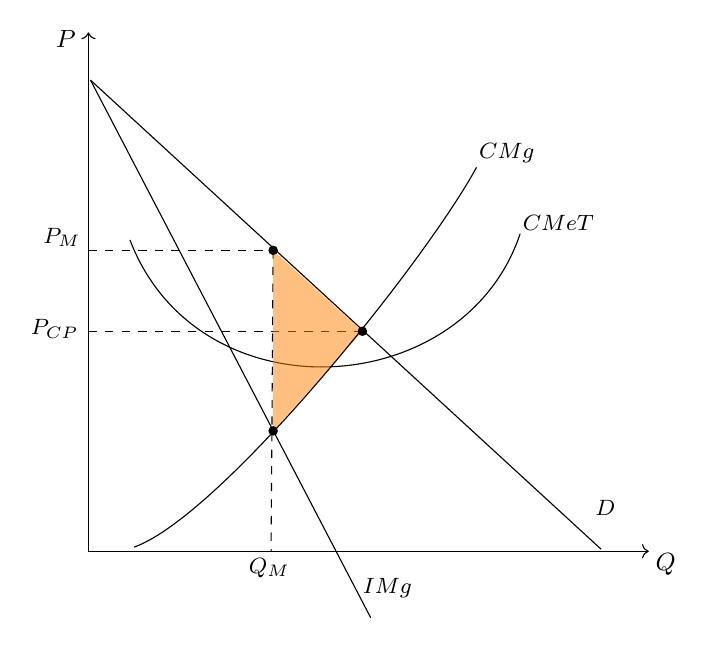
\begin{tikzpicture}[x=0.75pt,y=0.75pt,yscale=-1,xscale=1]

%Straight Lines [id:da6898288131267385] 
\draw[->]    (94,318) -- (364,318) ;
%Straight Lines [id:da9536118190051617] (eje Y)
\draw[->]    (94,318) -- (94,68) ;
%Straight Lines [id:da07757000222951138] (demanda)
\draw    (95,91) -- (341,317) ;
%Curve Lines [id:da3185207500621865] 
\draw    (114,168) .. controls (147,254) and (275,246) .. (302,165) ;
%Straight Lines [id:da9356870159511061] 
\draw[dashed]    (183,173) -- (182,318) ;
%Straight Lines [id:da6853761324294885] (IMg)
\draw    (95,91) -- (230,350) ;
%Straight Lines [id:da5731211677031389] 
\draw[dashed]    (94,173) -- (183,173) ;
%Straight Lines [id:da382163957096882] 
\draw[dashed]    (94,212) -- (226,212) ;


%Pérdida
\fill[orange, opacity=0.5] (183,173) -- (226,212) -- (183,260) -- cycle;


%Curve Lines [id:da24417480382196666] (CMg)
\draw    (116,316) .. controls (158,301) and (256,179) .. (281,133) ;

% Text Node
\draw (77,66) node [anchor=north west][inner sep=0.75pt]   [align=left] {\small $P$};
% Text Node
\draw (366,318) node [anchor=north west][inner sep=0.75pt]   [align=left] {\small $Q$};
% Text Node
\draw (302,155) node [anchor=north west][inner sep=0.75pt]   [align=left] {\footnotesize $CMeT$};
% Text Node
\draw (281,120) node [anchor=north west][inner sep=0.75pt]   [align=left] {\footnotesize $CMg$};
% Text Node
\draw (71,161) node [anchor=north west][inner sep=0.75pt]   [align=left] {\footnotesize $P_M$};
% Text Node
\draw (170,320) node [anchor=north west][inner sep=0.75pt]   [align=left] {\footnotesize $Q_M$};
% Text Node
\draw (65,205) node [anchor=north west][inner sep=0.75pt]   [align=left] {\footnotesize $P_{CP}$};
% Text Node
\draw (225,330) node [anchor=north west][inner sep=0.75pt]   [align=left] {\footnotesize $IMg$};
% Text Node
\draw (337,292) node [anchor=north west][inner sep=0.75pt]   [align=left] {\footnotesize $D$};

\filldraw (183,173) circle (1.5pt);
\filldraw (226,212) circle (1.5pt); %P_CP
\filldraw (183,260) circle (1.5pt);

\end{tikzpicture}
\end{frame}

\begin{frame}{Pérdida de eficiencia}
    \begin{itemize}
        \item El excedente total en la presencia
        de un monopolista es menor que en el caso de competencia perfecta, y la diferencia está dada por el \textcolor{orange}{triángulo naranja}.
        \item La mejora paretiana se alcanza si se redistribuye el excedente adicional de tal manera que alguno de los agentes esté mejor sin que el otro esté peor.
        \item Bajo monopolio, hay transacciones que no se terminan haciendo y que se hubiesen podido hacer en un contexto de competencia perfecta.
    \end{itemize}
    \begin{boxB}
    \centering
        El monopolio genera una pérdida de eficiencia puesto que transacciones deseables, que se llevarían a cabo en un contexto de competencia perfecta  (ya que el costo marginal es menor a la valoración del consumidor), no son realizadas.
    \end{boxB}
\end{frame}

\begin{frame}{Elasticidad y maximización}
    \begin{itemize}
    \item El margen de beneficios del monopolista depende de la elasticidad de la demanda a la que se enfrentan.
        \begin{itemize}
        \item  Cuanto más inelástica es la demanda, más puede aprovechar el monopolista  su poder de mercado. 
        \item Si la curva de demanda es perfectamente elástica, el monopolista se comporta como en competencia perfecta, no tiene poder de mercado. 
        \end{itemize}
    \end{itemize}
    \begin{boxB}
        \centering
        Mayor elasticidad $\Longrightarrow$ menor mark-up (menor poder de mercado)
    \end{boxB}
    \begin{itemize}
    \item La pérdida de eficiencia también depende entonces de la elasticidad:
        \begin{itemize}  
          \item  Cuanto más elástica es la demanda, más puede aprovechar el monopolista  su poder de mercado. 
         \end{itemize}
    \end{itemize}
    \begin{boxB}
    \centering
    Mayor elasticidad $\Longrightarrow$ menor pérdida de eficiencia 
    \end{boxB}
\end{frame}

\begin{frame}{La pérdida de eficiencia del
monopolio depende de la elasticidad de
la demanda}
\begin{center}
\begin{figure}[H]
\begin{center}
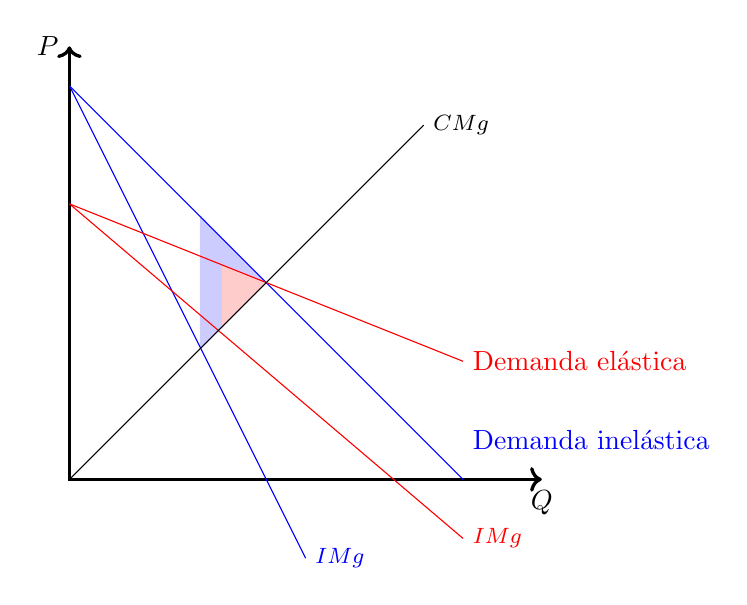
\begin{tikzpicture}[scale=0.5]
\draw[very thick,<->] (0,11) node[left]{$P$}--(0,0)--(12,0) node[below]{$Q$};
\draw[fill,blue!20] (5,5)--(3.33,3.32)--(3.33,6.7);
\draw[fill,red!20] (5,5)--(3.89,3.89)--(3.89,5.45);
\draw[thin, blue](0,10)--(10,0);
\draw[thin, blue](0,10)--(6,-2) node [right]{\footnotesize $IMg$} ;
\draw[thin,red](0,7)--(10,3) node[right]{Demanda elástica} ;
\draw[thin,red](0,7)--(10,-1.5)  node [right]{\footnotesize $IMg$} ;
\draw[thin](0,0)--(9,9) node [right]{\footnotesize $CMg$};
%\draw[thick,gray, dashed](0,4)--(4,4)--(4,0);
\node[right, blue] at (10,1){Demanda inelástica};
%\node[left]at (0,4){\footnotesize $P^*$};
%\node[below]at (8.3,1){\footnotesize $D$ };
  %\draw[fill] (4,4) circle [radius =0.1] node[above] {\scriptsize E};
  \end{tikzpicture}
\end{center}
\end{figure}
\end{center}
\end{frame}

\begin{frame}
\frametitle{Poder de mercado}
\begin{itemize}
    \item Vimos que el margen de beneficio de una empresa depende de la elasticidad de la demanda. \vspace{2mm}
        \item Esta, a su vez se ve afectada por la competencia:     
        \begin{itemize}
        \item Demanda relativamente inelástica si hay pocos sustitutos.
        \item Demanda de bienes esenciales o de primera necesidad también son más inelásticas.
        \item Las empresas con poder de mercado tienen suficiente poder de negociación para fijar los precios sin perder clientes. \vspace{2mm}
    \end{itemize}
    \item La política de competencia (\textit{antitrust}), que limita el poder de mercado, puede beneficiar a los consumidores. 
    \begin{itemize}
        \item Por ejemplo, evitar que empresas se pueden agrupar en un cartel (poniéndose de acuerdo para mantener precios altos).
        \item La reducción de costos de entrada también puede ser beneficiosa para los consumidores.
    \end{itemize}
\end{itemize}
\end{frame}

\begin{frame}{Un ejemplo}

\centering

\includegraphics[width=0.75\textwidth]{Slides Principios de Economia/Figures/Magistral_15/M15.3.jpg}

\end{frame}

\begin{frame}
\frametitle{¿Cómo ganan poder de mercado las empresas?}
\begin{itemize}
    \item La innovación tecnológica permite diferenciar los productos.
    \begin{itemize}
        \item Crear productos distintos en calidad, diseño, funciones, rendimiento, etc. Apple innovó con el iPhone introduciendo funciones exclusivas (Face ID, ecosistema iOS).
        \item Una empresa que inventa un producto completamente nuevo pueden prevenir la competencia a través de patentes o las leyes de copyright. \vspace{1mm}
  \end{itemize}
        \item Con la publicidad las empresas pueden atraer a los consumidores, alejándolos de la competencia y creando lealtad a la marca. \vspace{1mm}
        \item Ambas tácticas pueden cambiar la curva de demanda que enfrenta la empresa. 
\end{itemize}
\end{frame}

\begin{frame}
\frametitle{Monopolios naturales}
\begin{itemize}
    \item Hay casos en los cuales el poder monopólico surge de características tecnológicas, de estructura de costos.\vspace{1mm}
    \item El costo marginal es constante y muy bajo. \vspace{1mm}
    \item El costo medio es decreciente. 
        \begin{itemize}
            \item Economías de escala, altos costos fijos, o precios de factores que caen cuanto más compra la empresa.
            \item Los altos costos fijos imponen barreras a la entrada. \vspace{1mm}
        \end{itemize}
        \item La empresa debe elegir un precio al menos igual al costo medio, que es más alto que el costo marginal. 
        \begin{itemize}
            \item ¿Por qué? \vspace{1mm}
        \end{itemize}
        \item En estos casos tenemos un monopolio natural.
        \begin{itemize}
            \item En lugar de fomentar la competencia, el gobierno suele poner controles de precios o hacer estas empresas de propiedad pública.
        \end{itemize}
    \end{itemize}
\end{frame}


\begin{frame}
\frametitle{Monopolio natural}
\begin{figure} [H]
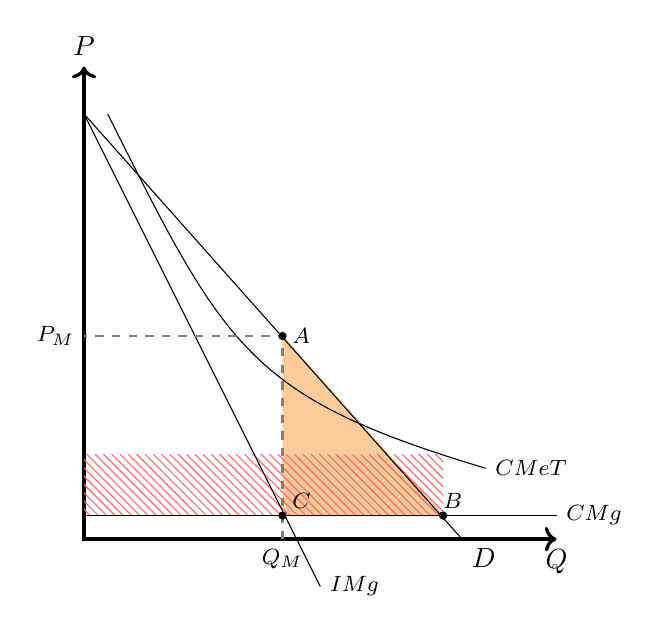
\begin{tikzpicture}[scale=0.6]
\draw[very thick,<->] (0,10) node[above]{$P$}--(0,0)--(10,0) node[below]{$Q$};

\node[left] at (0,4.3) {\footnotesize $P_M$};
\node[below] at (4.2,0) {\footnotesize $Q_M$};
%\node[left] at (0,1.2) {\footnotesize $P_R$};

\draw[fill,orange!40] (4.2,4.3)--(7.6,0.5)--(4.2,0.5);

\fill[pattern=north west lines, pattern color=red!60] (0,0.5) rectangle (7.6,1.8);

%\node[right] at (5.65,2.75) {\footnotesize $B$};
%\node[below] at (7.9,0) {\footnotesize $C$};
\draw[thin](0,9)--(8,0) node[below right]{$D$};
\draw[thin](0,9)--(5,-1) node[right]{\footnotesize $IMg$};
\draw[thin](0,0.5)--(10,0.5) node[right]{\footnotesize $CMg$};
\draw[thin](0.5,9) ..controls (3,4) and (3.5,3) .. (8.5,1.5) node[right]{\footnotesize $CMeT$};
\draw[thick, dashed,gray] (4.2,0)--(4.2,4.3)--(0,4.3);

\fill (4.2,4.3) circle (2.5pt);
\node[right] at (4.2,4.3) {\footnotesize $A$};

\fill (7.6,0.5) circle (2.5pt);
\node[right] at (7.4,0.8) {\footnotesize $B$};

\fill (4.2,0.5) circle (2.5pt);
\node[right] at (4.2,0.8) {\footnotesize $C$};

\end{tikzpicture}
\end{figure} 
\end{frame}


\begin{frame}
\frametitle{Casos ideales}
\small
\begin{center}
\renewcommand{\arraystretch}{1.3} % Espaciado entre filas
    \setlength{\tabcolsep}{6pt} % Espaciado entre columnas
    \rowcolors{2}{white!100}{white!95} % Alternar colores de filas
    \newcolumntype{P}{>{\centering\arraybackslash}p{4.5cm}}
    \begin{tabular}{P|P}
    \hline
    \rowcolor{blue!20} % Color de fondo del encabezado
    Tomadores de precios & Fijadores de precio \\
    \rowcolor{blue!20} % Color de fondo del encabezado
    \textbf{Competencia Perfecta} & \textbf{Monopolio}
    \\
    \hline
    Puede ser Pareto  & Pareto ineficiente \\ 
    eficiente & (pérdidas peso muerto) \\
    \hline
    No hay rentas económicas & Rentas económicas tanto \\
    en el largo plazo & a largo como a corto plazo \\
    \hline
    Poca gasto en su & Firmas publicitan \\ publicidad & producto único 
    \\
    \hline
    Pocos incentivos para innovar & Firmas invierten en IyD \\ 
    porque otras van a copiar & (tratan de evitar ser copiadas)
\end{tabular}
\end{center}
\end{frame}

\begin{frame}
\frametitle{Competencia imperfecta}
\begin{itemize}
    \item La empresa típica se ubica en algún punto entre los casos extremos de la competencia perfecta y el monopolio. \vspace{2mm}
    \item Mercados de competencia imperfecta: \vspace{1mm}
    \begin{itemize}
        \item \textbf{Oligopolio}
        \begin{itemize}
        \item Solo hay pocos vendedores.
        \item Se ofrece un producto idéntico o similar a los productos ofrecidos por otros vendedores.
        \item Las empresas deben tener en cuenta las reacciones de sus competidoras a los cambios de precios.
        \item Ejemplos: OPEP, Movistar/Personal/Claro. 
        \end{itemize} 
        \vspace{1mm}
        \item \textbf{Competencia monopolística}
        \begin{itemize}
        \item Hay muchos vendedores.
        \item Se ofrecen productos diferenciados (cada empresa enfrenta una curva de la demanda con pendiente negativa).
        \item Hay libertad para entrar y salir del mercado. 
        \item Ejemplos: McDonald's/Burger King, CocaCola/Pepsi, marcas de ropa.
         \end{itemize} 
    \end{itemize}
    \end{itemize}
\end{frame}


\begin{frame}{Clasificación de las estructuras de mercado}

\centering
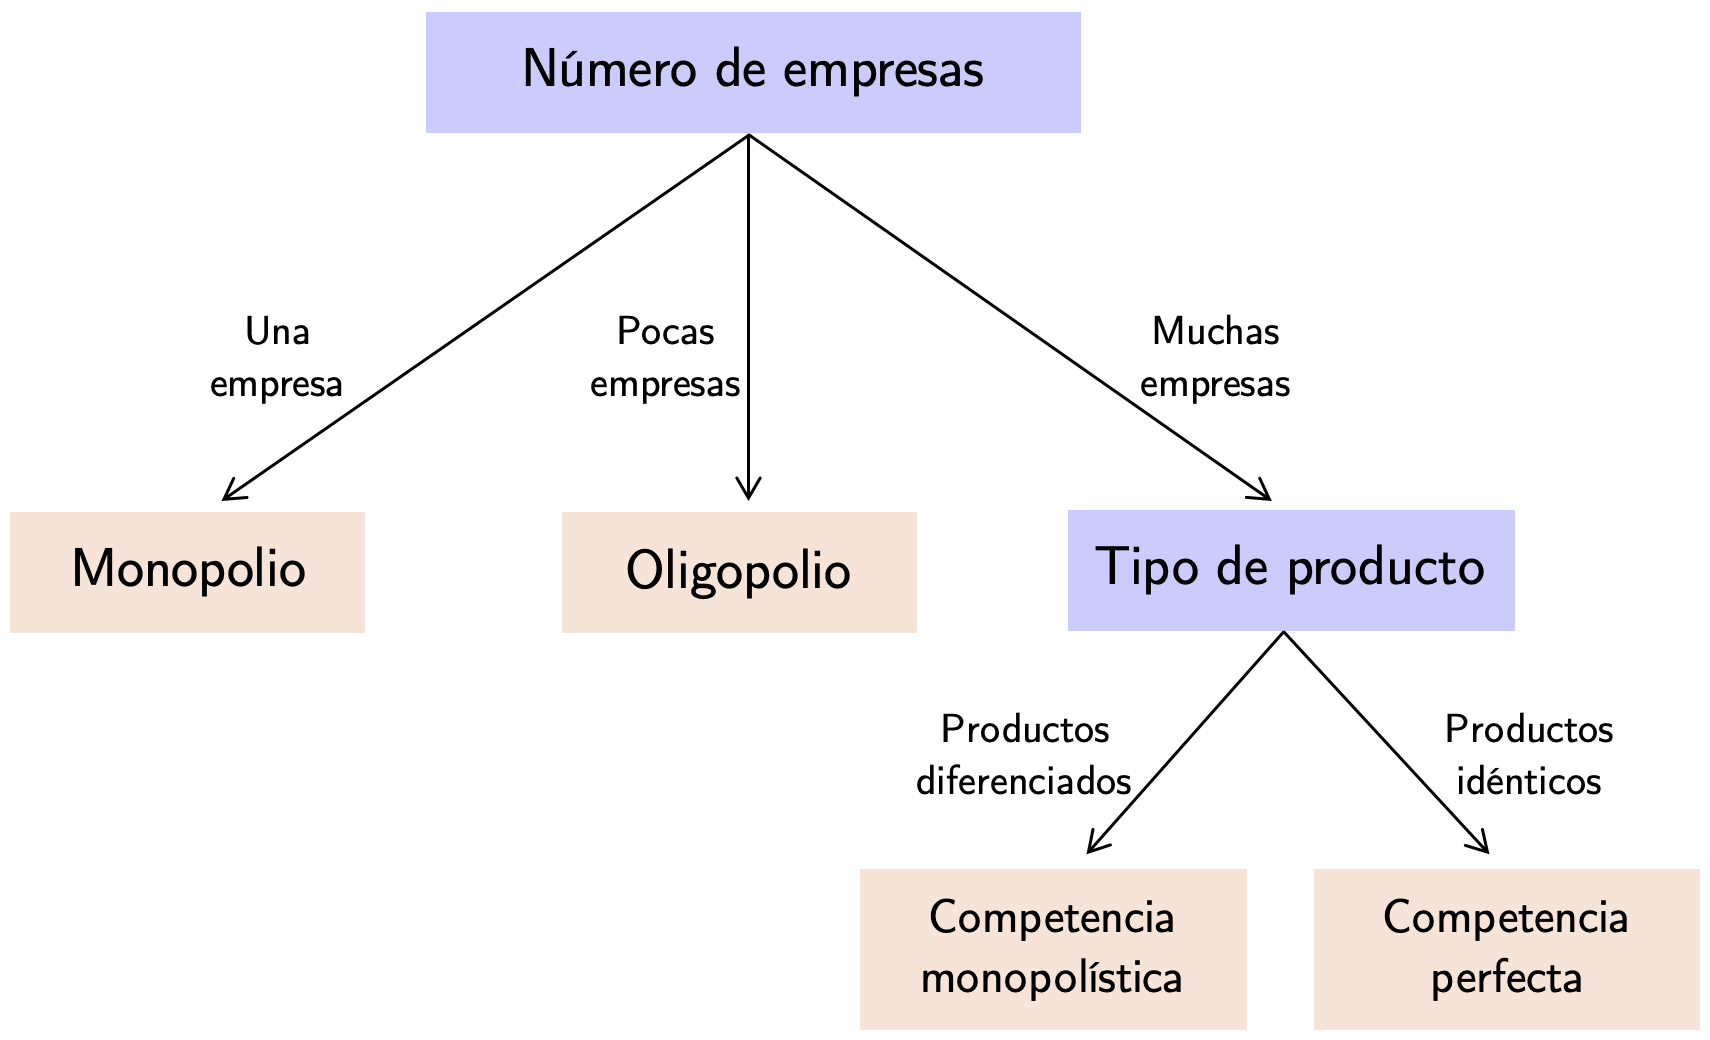
\includegraphics[width=0.95\textwidth]{Slides Principios de Economia/Figures/Magistral_15/Tipos_mercados.jpg}

\end{frame}

\begin{frame}
\frametitle{Determinantes de la concentración}
\begin{itemize}
    \item Costos:
        \begin{itemize}
        \item La existencia de economías de escala hace que solo sobrevivan en el mercado pocas empresas produciendo una gran parte de lo que demanda el mercado. 
        \end{itemize}
    \vspace{2mm}
    \item Barreras a la entrada:
        \begin{itemize}
        \item Cuando hay barreras a la entrada se bloquea el acceso para que otros empresas ingresen al mercado (concesiones estatales, requisitos de capital, barreras estratégicas o tecnológicas). 
        \end{itemize}
    \vspace{2mm}
    \item Interdependencia estratégica:
        \begin{itemize}
        \item Cuando las decisiones de una empresa dependen de las decisiones que toman otras empresas.
        \end{itemize}
    \end{itemize}
\end{frame}

\begin{frame}{¿Concentración en Argentina?}

\centering
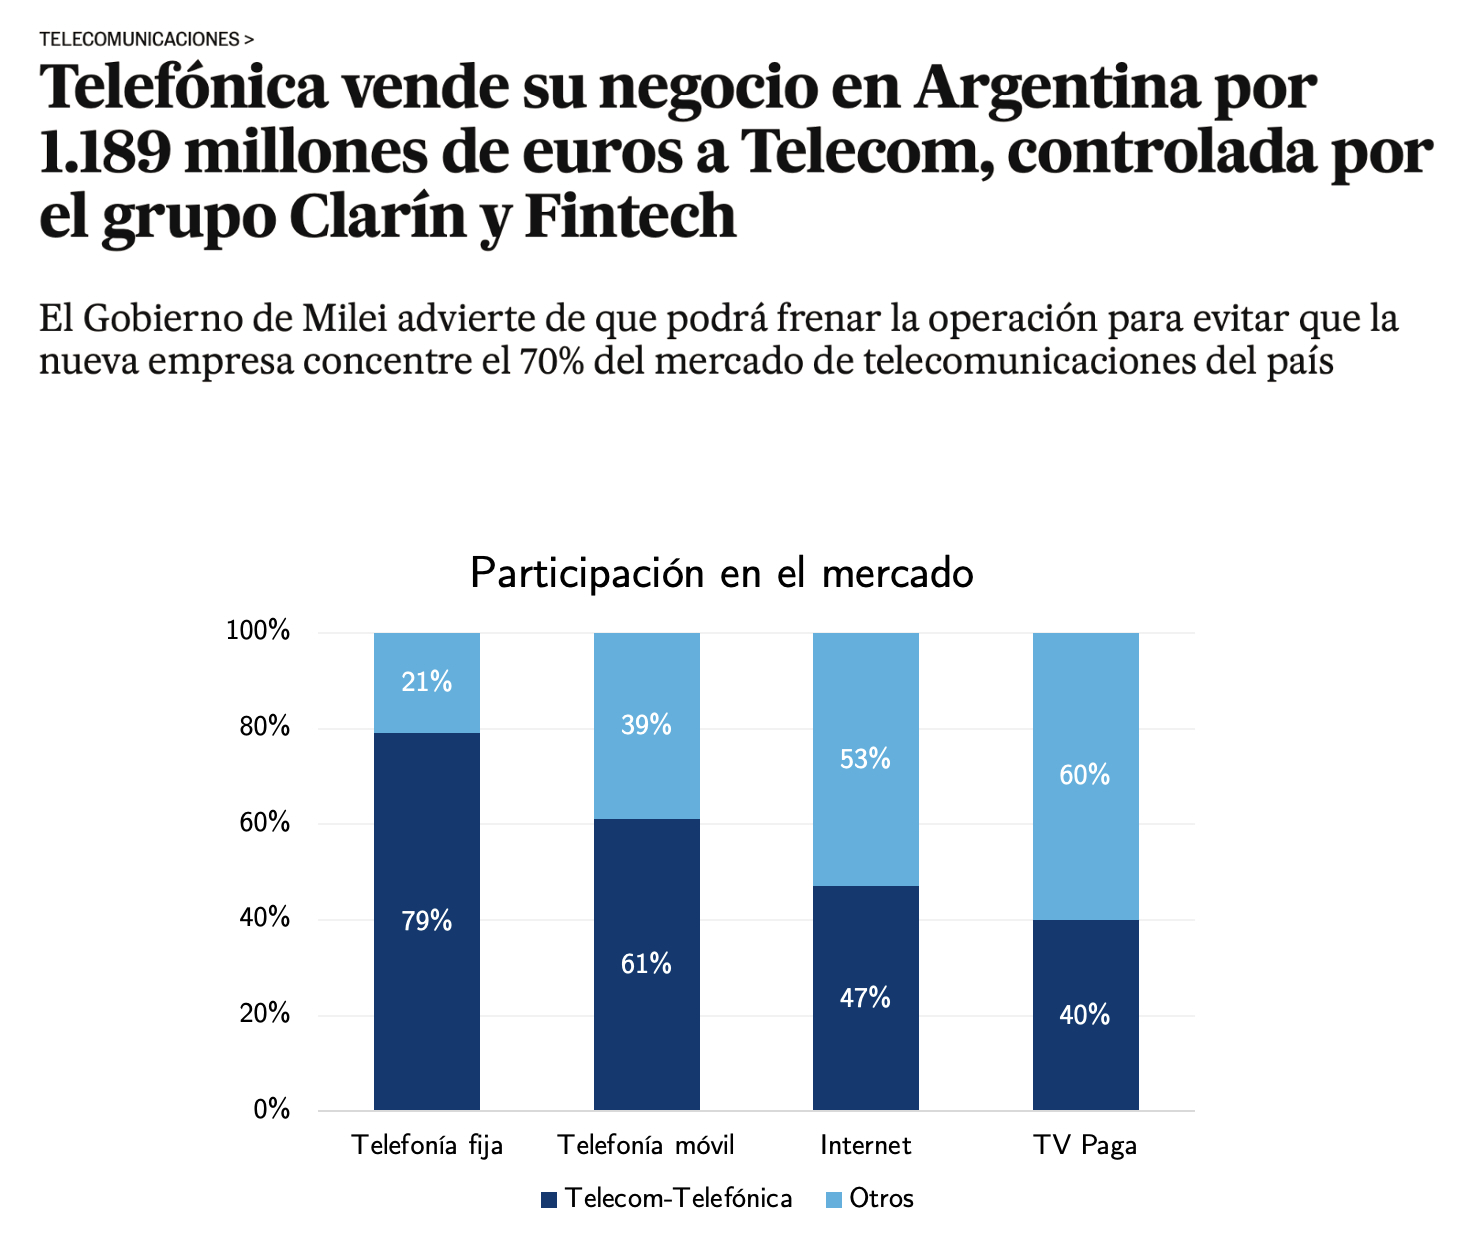
\includegraphics[width=0.75\textwidth]{Slides Principios de Economia/Figures/Magistral_15/M15.2.jpg}

\end{frame}


\begin{frame}{¿Concentración en Argentina?}

\centering
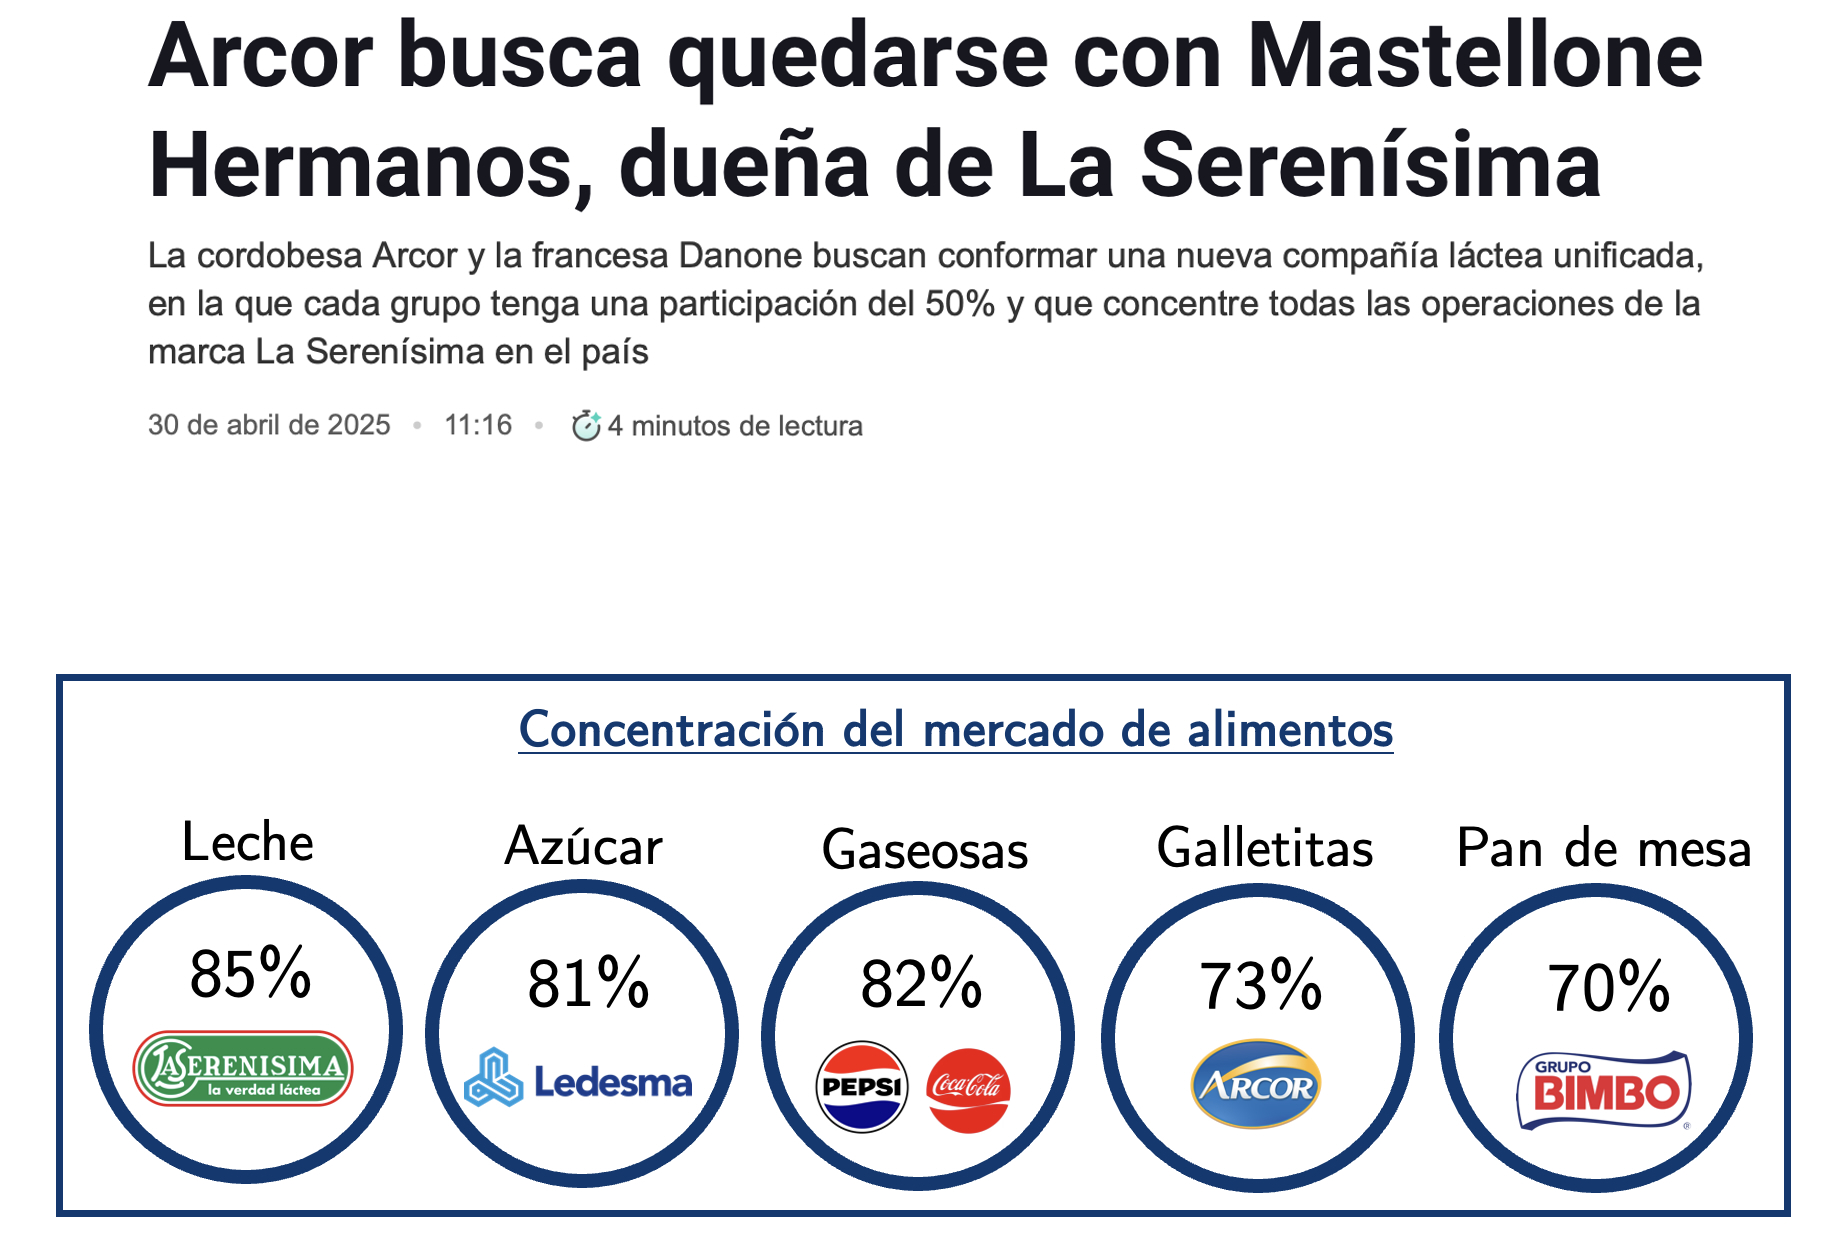
\includegraphics[width=0.85\textwidth]{Slides Principios de Economia/Figures/Magistral_15/M15.4.jpg}


\end{frame}

%\begin{frame}
%\frametitle{El caso de las cementeras}
%\centering
%
\includegraphics[width=0.95\textwidth]{Slides Principios de Economia/Figures/Cartel.png}
%\end{frame}

%\begin{frame}
%\frametitle{Competencia monopolística}
%\begin{center}
%  \href{https://www.youtube.com/watch?v=po0jY4WvCIc}{    
\includegraphics[width=0.75\textwidth]{Slides Principios de Economia/Figures/Diferenciacion (1).png}}
%\end{center}
%\end{frame}


%\begin{frame}
%\frametitle{La maximización de beneficios en Competencia Monopolística en corto plazo}
%\centering
%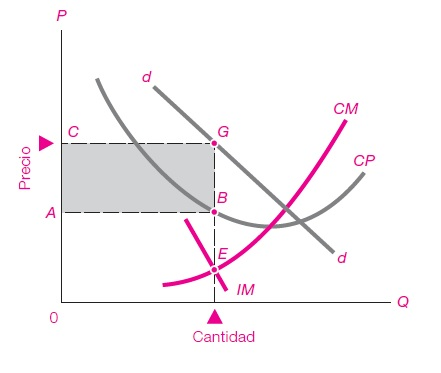
\includegraphics[scale=0.75]{Slides Principios de Economia/Figures/Tema_08.01_compmonop.jpg}

%\begin{figure}[h!]
%\renewcommand{\figurename}{Figure}

%\tikzset{every picture/.style={line width=0.75pt}} %set default line width to 0.75pt        
%\begin{center}
%\begin{tikzpicture}[x=0.75pt,y=0.75pt,yscale=-1,xscale=1]
% \path (0,1278); %set diagram left start at 0, and has height of 1278

%Straight Lines Eje
%\draw    (94,318) -- (364,318) ;
%\draw [shift={(366,318)}, rotate = 180] [color={rgb, 255:red, 0; green, 0; blue, 0 }  ][line width=0.75]    (10.93,-3.29) .. controls (6.95,-1.4) and (3.31,-0.3) .. (0,0) .. controls (3.31,0.3) and (6.95,1.4) .. (10.93,3.29)   ;
%Straight Lines: Eje
%\draw    (94,318) -- (94,68) ;
%\draw [shift={(94,66)}, rotate = 450] [color={rgb, 255:red, 0; green, 0; blue, 0 }  ][line width=0.75]    (10.93,-3.29) .. controls (6.95,-1.4) and (3.31,-0.3) .. (0,0) .. controls (3.31,0.3) and (6.95,1.4) .. (10.93,3.29)   ;

% Membrete eje Y
%\draw (77,46) node [anchor=north west][inner sep=0.75pt]   [align=left] {$p$};
% Membrete eje X
%\draw (366,318) node [anchor=north west][inner sep=0.75pt]   [align=left] {$q$};


% AR 
%\draw    (95,91) -- (330,310) ;
%\draw (320,290) node [anchor=north west][inner sep=0.75pt]   [align=left] {Demanda};
% Img (MR)
%\draw    (95,91) -- (240,317) ;
%\draw (240,300) node [anchor=north west][inner sep=0.75pt]   [align=left] {Img};
% dash lines
%\draw[thick, dashed, gray] (94,193)-- (202,193) -- (202,320);
%\node [below] at (200,318) {$q_1$};
%Shape: Rectangle profit
%\draw  [fill={rgb:red,4;green,2;yellow,1 }  ,fill opacity=0.48 ] (94,193) -- (202,193) -- (202,220) -- (94,220) ;
%\draw (72,190) node [anchor=north west][inner sep=0.75pt]   [align=left] {$p_1$};
%Curve Lines Cme T 
%\draw    (135,158) .. controls (147,269) and (280,210) .. (302,165) ;
%\draw (302,165) node [anchor=north west][inner sep=0.75pt]   [align=left] {CmeT};
% curve line Cmg
%\draw    (116,290) .. controls (158,355) and (250,179) .. (281,133) ;
%\draw (281,133) node [anchor=north west][inner sep=0.75pt]   [align=left] {Cmg};

% short run equilibrium

%\draw[thin, ->] (170,202).. controls (210,180) and         %(210,185)..(219,175);
%\node[right] at (190,165) {\footnotesize Beneficio};

%\end{tikzpicture}
%\end{center}
%\end{figure}
%\end{frame}

%\begin{frame}
%\frametitle{Competencia monopolística en el largo plazo}
%\begin{itemize}
%    \item Los beneficios positivos en el corto plazo atraen nuevas empresas.\vspace{2mm}
%    \item La demanda que enfrenta la empresa se contrae.\vspace{2mm}
%    \item Los precios son superiores a los costos marginales.\vspace{2mm}
%    \item En el largo plazo, los beneficios de la empresa son iguales a cero, es decir, tiene beneficios normales.
%\end{itemize}
%\end{frame}

%\begin{frame}
%\frametitle{La maximización de beneficios en Competencia Monopolística en largo plazo}
%\centering
%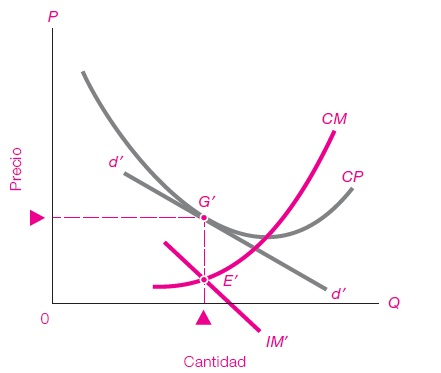
\includegraphics[scale=0.7]{Slides Principios de Economia/Figures/Tema_08.02_compmonop.jpg}

%\begin{figure}[H]
%\renewcommand{\figurename}{Figure}
%\begin{tikzpicture}[scale=0.45]
%\centering
%\tikzset{every picture/.style={line width=0.75pt}} %set default line width to 0.75pt        
%\begin{center}
%\begin{tikzpicture}[x=0.75pt,y=0.75pt,yscale=-1,xscale=1]
% \path (0,1278); %set diagram left start at 0, and has height of 1278

%Straight Lines [id:da6898288131267385] 
%\draw    (94,318) -- (364,318) ;

%\draw [shift={(366,318)}, rotate = 180] [color={rgb, 255:red, 0; green, 0; blue, 0 }  ][line width=0.75]    (10.93,-3.29) .. controls (6.95,-1.4) and (3.31,-0.3) .. (0,0) .. controls (3.31,0.3) and (6.95,1.4) .. (10.93,3.29)   ;
%Straight Lines [id:da9536118190051617] 
%\draw    (94,318) -- (94,68) ;
%\draw [shift={(94,66)}, rotate = 450] [color={rgb, 255:red, 0; green, 0; blue, 0 }  ][line width=0.75]    (10.93,-3.29) .. controls (6.95,-1.4) and (3.31,-0.3) .. (0,0) .. controls (3.31,0.3) and (6.95,1.4) .. (10.93,3.29)   ;
% AR 
%\draw    (95,91) -- (201,317) ;
%\draw (200,300) node [anchor=north west][inner sep=0.75pt]   [align=left] {Demanda};
% Img (MR)
%\draw    (95,91) -- (150,317) ;
%\draw (155,300) node [anchor=north west][inner sep=0.75pt]   [align=left] {Img};
% dash lines
%\draw[thick, dashed, gray] (94,191)-- (146,191) -- (146,320);
%\node [below] at (146,318) {$q_1$};
%\draw (72,191) node [anchor=north west][inner sep=0.75pt]   [align=left] {$p_1$};
%Shape: Rectangle profit
%\draw  [fill={rgb:red,4;green,2;yellow,1 }  ,fill opacity=0.48 ] (94,193) -- (202,193) -- (202,220) -- (94,220) ;


%Curve Lines Cme T 
% MAS ALEJADA LA CME T
%\draw    (180,128) .. controls (147,200) and (280,210) .. (302,165) ;
%\draw (302,165) node [anchor=north west][inner sep=0.75pt]   [align=left] {CmeT};
% MISMA QUE LA DE SHORT RUN
%\draw    (135,158) .. controls (147,269) and (280,210) .. (302,165) ;
%\draw (302,165) node [anchor=north west][inner sep=0.75pt]   [align=left] {CmeT};

% curve line Cmg
%\draw    (116,290) .. controls (158,355) and (250,179) .. (281,133) ;
%\draw (281,133) node [anchor=north west][inner sep=0.75pt]   [align=left] {Cmg};

% Text Node
%\draw (77,46) node [anchor=north west][inner sep=0.75pt]   [align=left] {$p$};
% Text Node
%\draw (366,318) node [anchor=north west][inner sep=0.75pt]   [align=left] {$q$};

% Long run equilibrium
%\draw[thin, ->] (150,191).. controls (190,160) and         (210,125)..(210,125);
%\node[right] at (200,100) {\footnotesize Equilibrio de};
%\node[right] at (200,115) {\footnotesize largo plazo};

%\end{tikzpicture}
%\end{center}
%\end{figure}

%\end{frame}
\end{document}
